\documentclass{powerdot}

\pdsetup{lf={Jordan Thayer (Draper)},
	 rf={15 Puzzle}}

% for including postscript
\usepackage{graphicx}
\usepackage{amsmath}
\usepackage{latexsym} %%box def
\usepackage{pstricks,,pst-node,pst-tree}
\usepackage{amssymb}
\DeclareMathOperator*{\argmin}{argmin}
% get my macros

% shorthand for including the figures
\newcommand{\figwidth}[1]{%
	\bc
	\includegraphics[width=\textwidth]{#1}
	\ec
}
\newcommand{\figheight}[1]{%
	\bc
	% height=2.8in
	\includegraphics[height=2.8in]{#1}
	\ec}

\newcommand{\qspace}{\vspace{0.1in}}
\newcommand{\myred}[1]{{\color{red} #1}}
\newcommand{\mygreen}[1]{{\color{green} #1}}
\newcommand{\myyellow}[1]{{\color{yellow} #1}}
\newcommand{\turnred}[1]{{\onslide*{1}{#1}\onslide*{2}{\color{red} #1}}}
\newcommand{\myblue}[1]{{\color{blue} #1}}

\newcommand{\mybf}[1]{\textcolor{red}{\bf #1}}
\newcommand{\myem}[1]{\textcolor{blue}{\em #1}}
\newcommand{\openfH}{{\myit open}_{\widehat{f}}}
\newcommand{\openf}{{\myit open}_f}


\title{AI For Games: What Are We Talking About?}
\author{Jordan Thayer}

\date{\vspace{0.2in}}
\begin{document}
\maketitle

\section[slide=false]{Logistics}
\begin{slide}{Syllabus}
  \begin{enumerate}
    \item Introduction To Games
      \subitem Syllabus
      \subitem Types of Games
      \subitem Terminology
      \subitem Brief History of Games and AI
    \item Minimax Tree Search
    \item $\alpha$-$\beta$ pruning
    \item Multi-Armed Bandits and Monte Carlo Tree Search
    \item Implementing Monte Carlo Tree Search
    \item Weak and Strong Solutions to Games, Checkers
  \end{enumerate}
\end{slide}

\begin{slide}{Today\hfill Multi-Armed Bandits and Monte Carlo Tree Search}
  \begin{itemize}
    \item One Armed Bandits
    \item Distribution Estimation
    \item More than One Arm
    \item Formalizing Regret
    \item Transformation to Trees
  \end{itemize}
\end{slide}

%%%%%%%%%%%%%%%%%%%%%%%%%%%%%%%%%%%%%%%%%%%%%%%%%%%%%%%%%%%%%%%%%%%
\section{Distribution Estimation}

\begin{slide}{Bandit Games}

  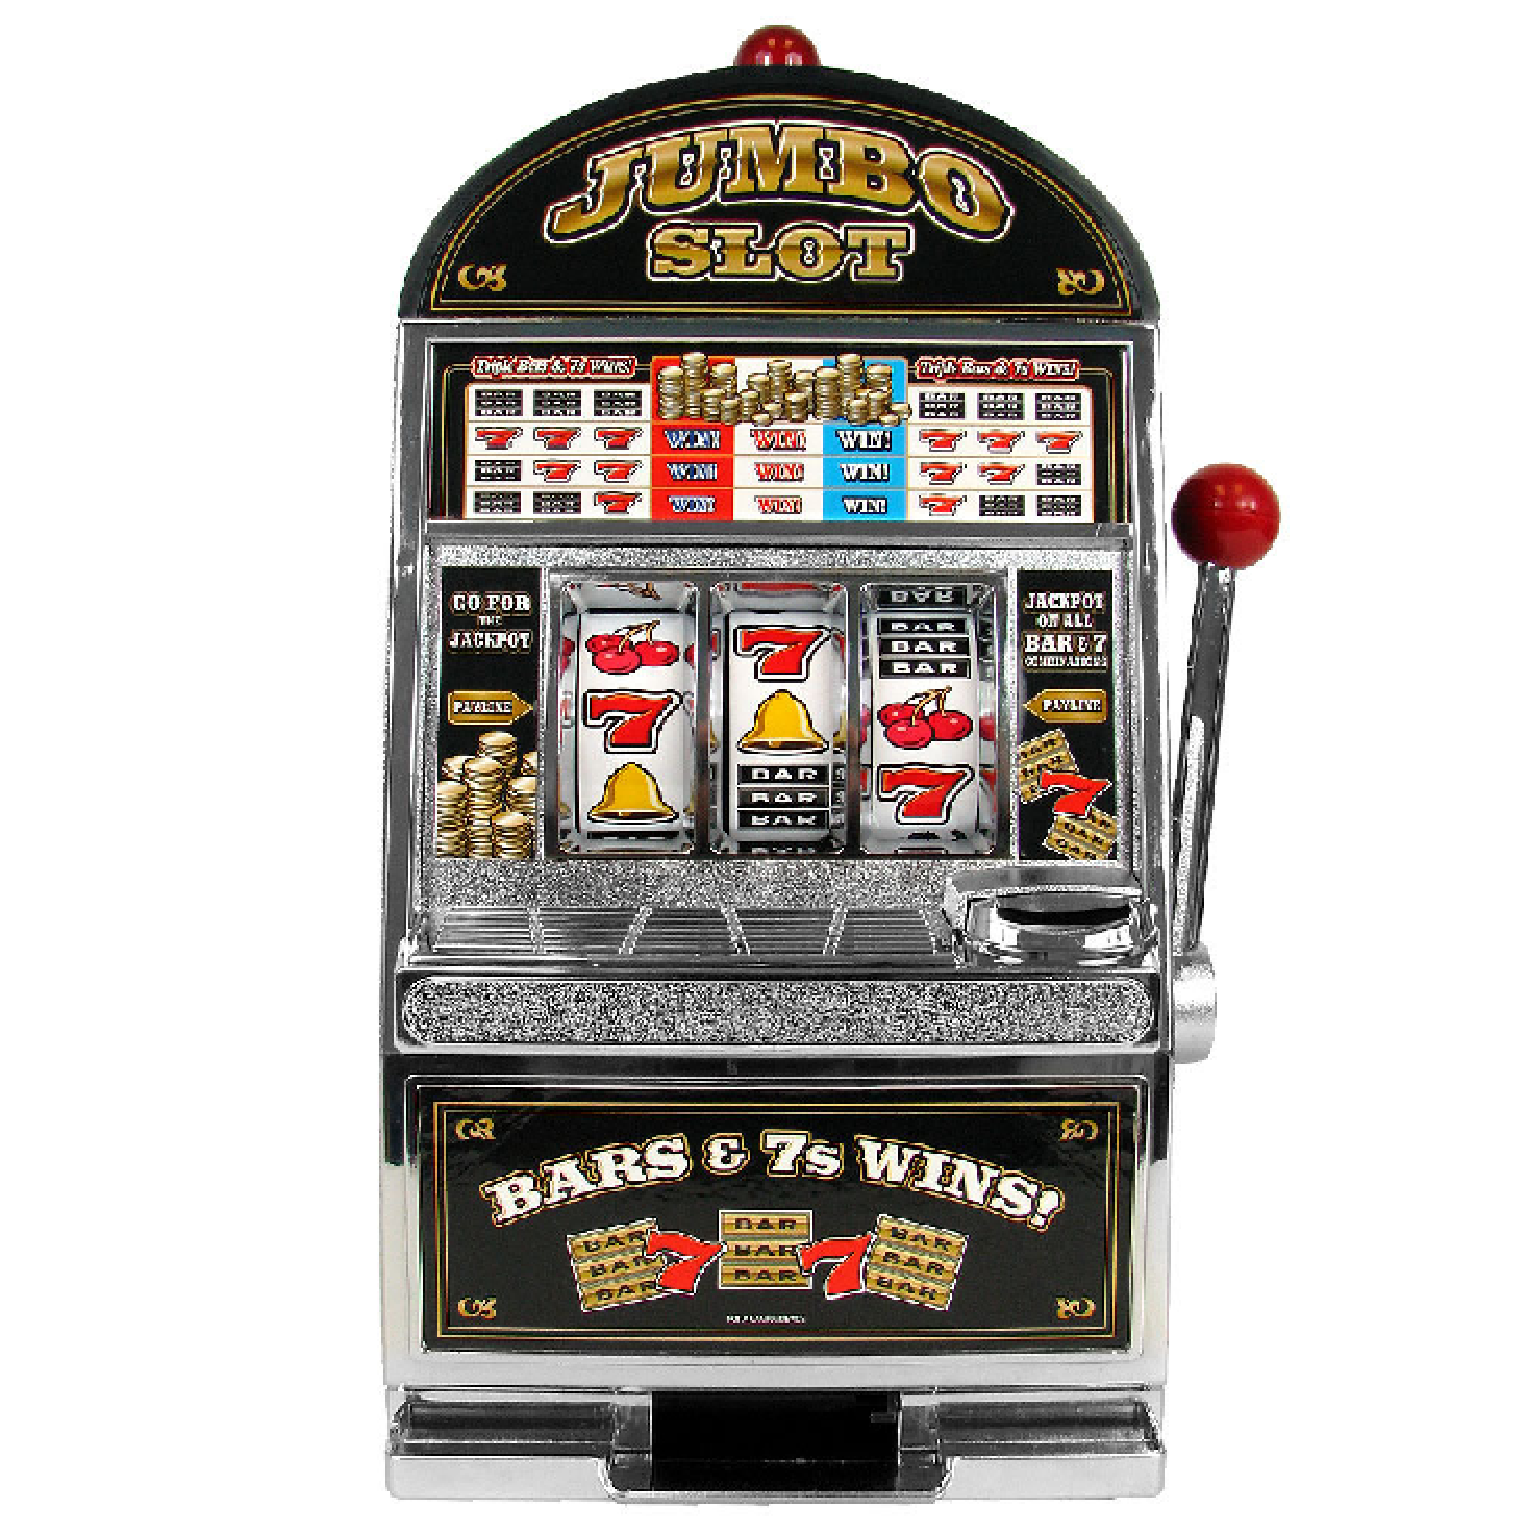
\includegraphics[width=3in]{images/one-armed-bandit.eps}

\end{slide}

\begin{slide}{Distribution Estimation}
  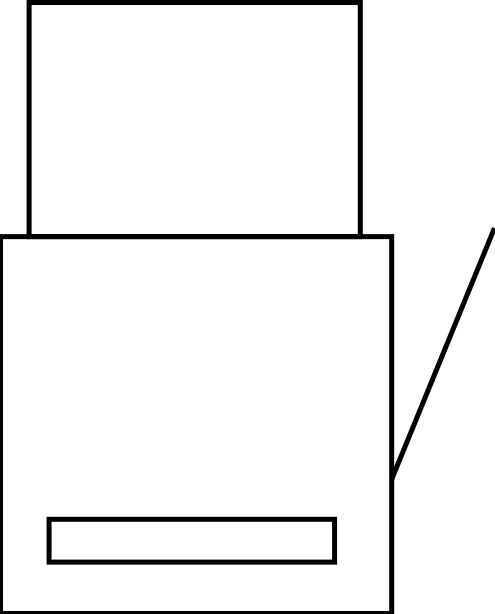
\includegraphics[width=2in]{images/one_bandit.eps}
\end{slide}
  %% First payout
\begin{slide}[toc=]{Distribution Estimation}
  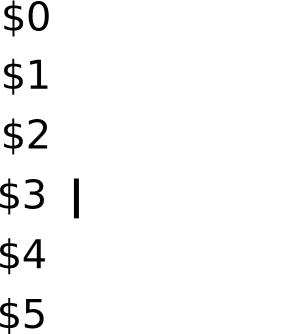
\includegraphics[width=0.75in]{images/discret_dist_1.eps}
  %% second payout
\end{slide}

\begin{slide}[toc=]{Distribution Estimation}
  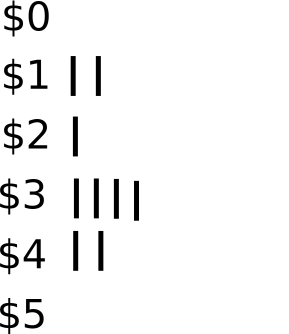
\includegraphics[width=1in]{images/discret_dist_2.eps}
  %% third payout, same as first
\end{slide}

\begin{slide}[toc=]{Distribution Estimation}
  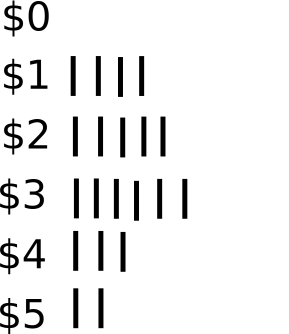
\includegraphics[width=1in]{images/discret_dist_3.eps}
\end{slide}
  %% ...
  %% Hey look it's a distribution!
\begin{slide}[toc=]{Distribution Estimation}
  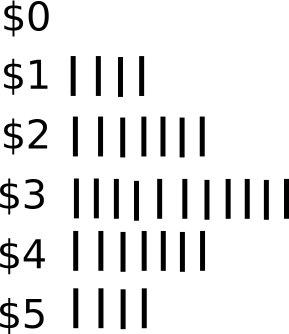
\includegraphics[width=2in]{images/discret_dist_end.eps}
\end{slide}

\begin{slide}[toc=]{Distribution Estimation}
  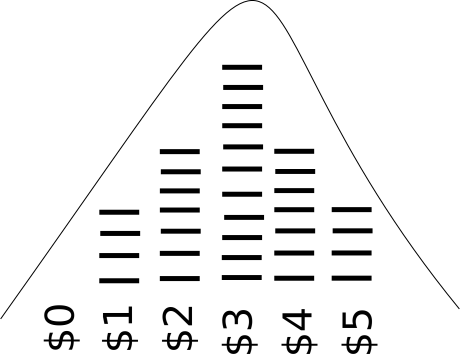
\includegraphics[width=\textwidth]{images/discret_dist_as_dist.eps}
\end{slide}

\begin{slide}{Formally}
  Let's say we have a model of our distribution:\\
  $ f(x | \mu, \sigma^2)= \frac{1}{\sigma \sqrt{2\pi}} e^{-
    \frac{(x-\mu)^2}{2\sigma^2}}$\\\pause
  \vspace{0.2in}
  Further, we have a source of data:\\ %% Picture of the bandit
  \begin{center}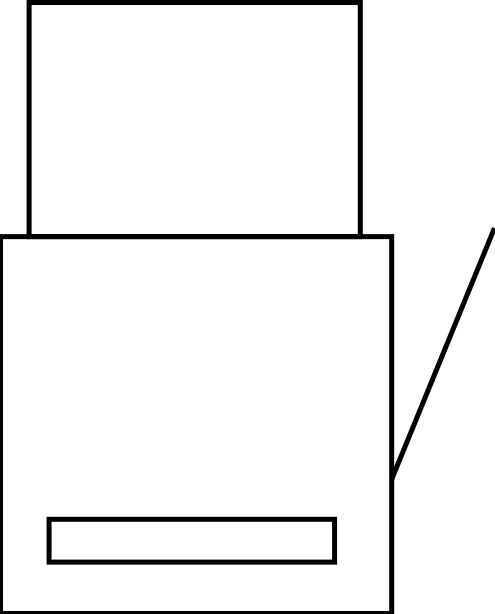
\includegraphics[height=0.5in]{images/one_bandit.eps}\end{center}\pause
  Now, we just need to divine $\mu$ and $\sigma$ by sampling from the data.\\ %% picture of lady playing slots

  $\mu = \frac{1}{n} \sum_{i=1}^{n} payout_i$\\
  $\sigma^2 = \frac{1}{n} \sum_{i=1}^{n} (payout_i - \mu)^2$
\end{slide}

%%%%%%%%%%%%%%%%%%%%%%%%%%%%%%%%%%%%%%%%%%%%%%%%%%%%%%%%%%%%%%%%%%%
\section{Multiple Arms, Regret}
\begin{slide}{Going from 1 to n}
  %% Show single machine
  \onslide*{1}{
    Before, we had a single machine.\\
    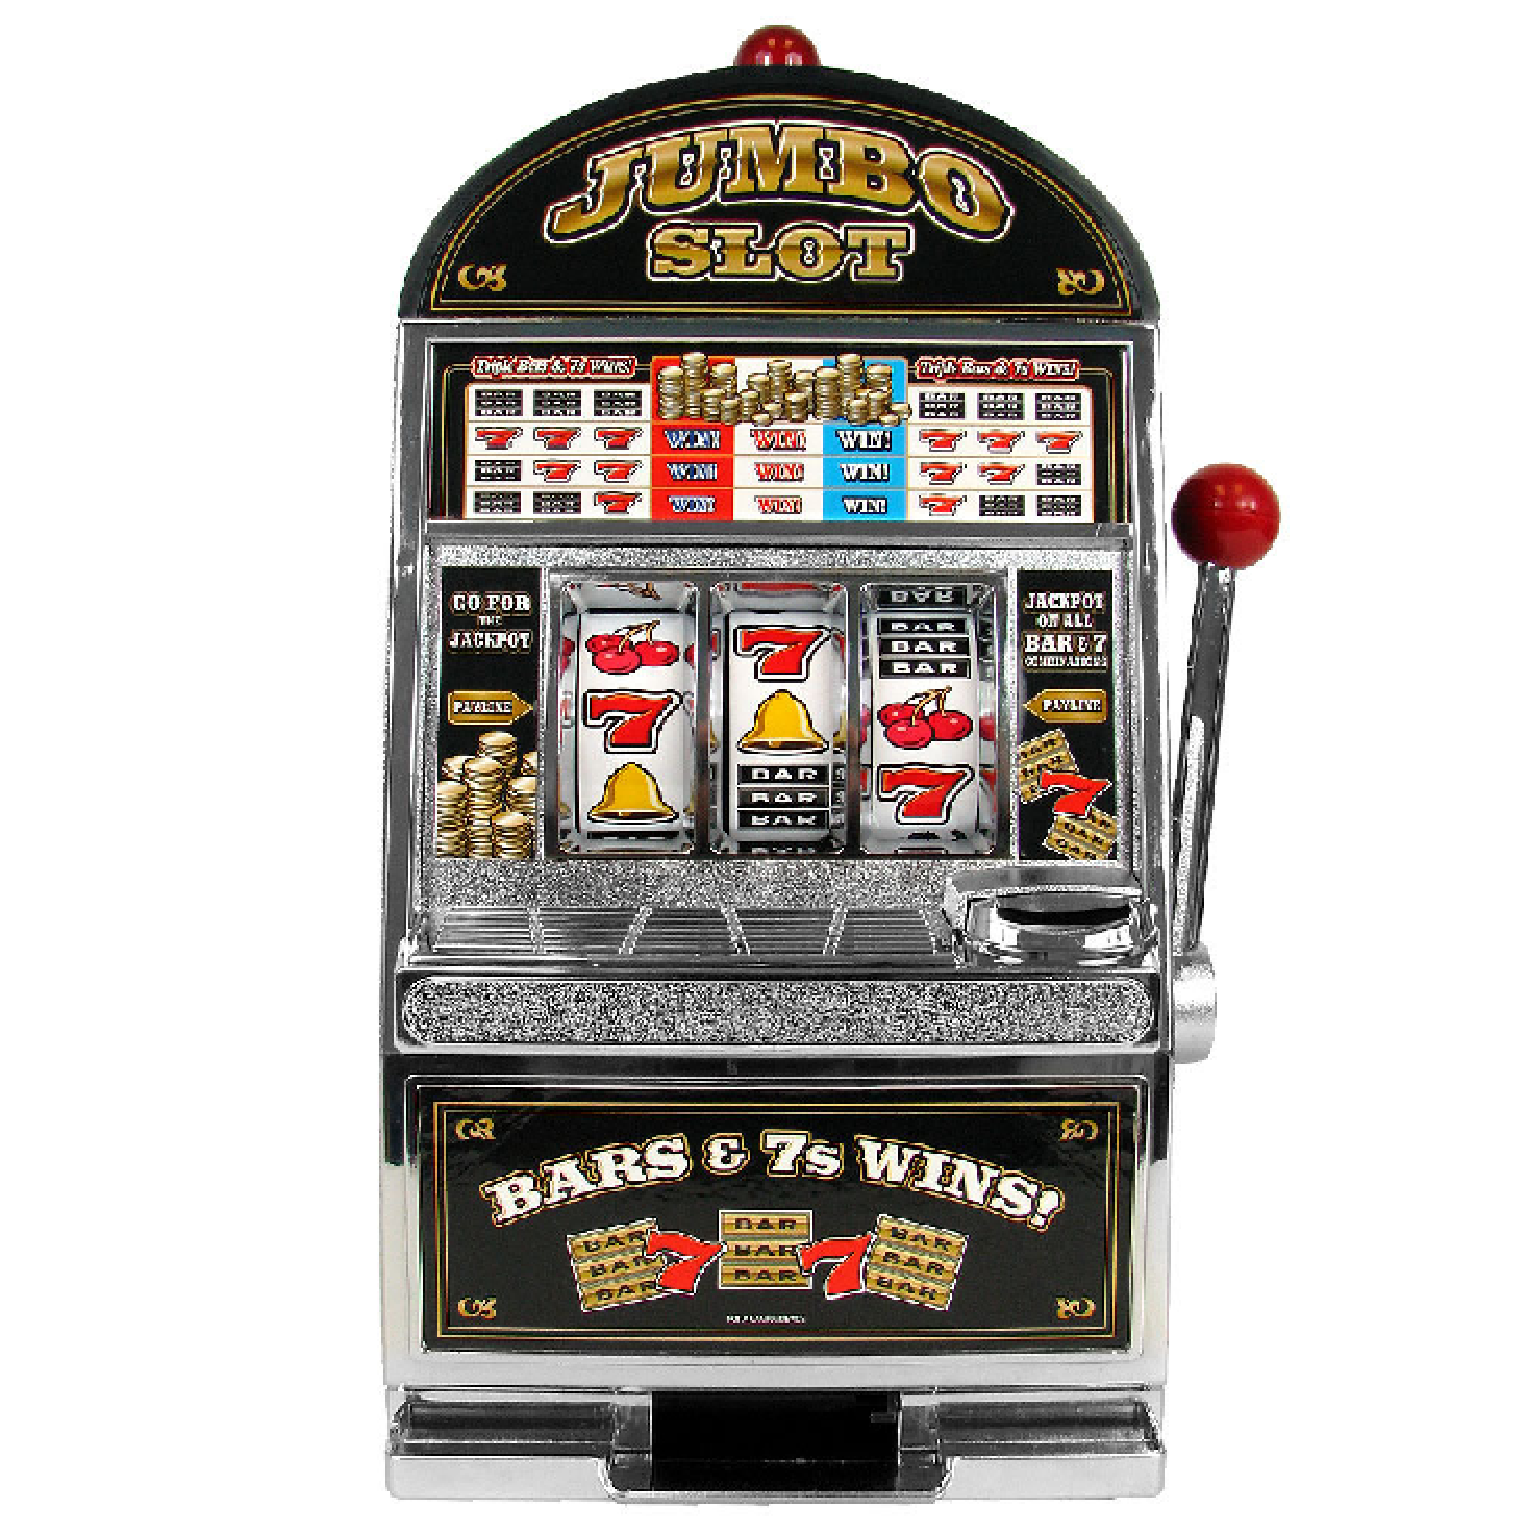
\includegraphics[width=3in]{images/one-armed-bandit.eps}
  }
  %% show an actual casion row
  \onslide*{2}{
    But that isn't what's normal.
    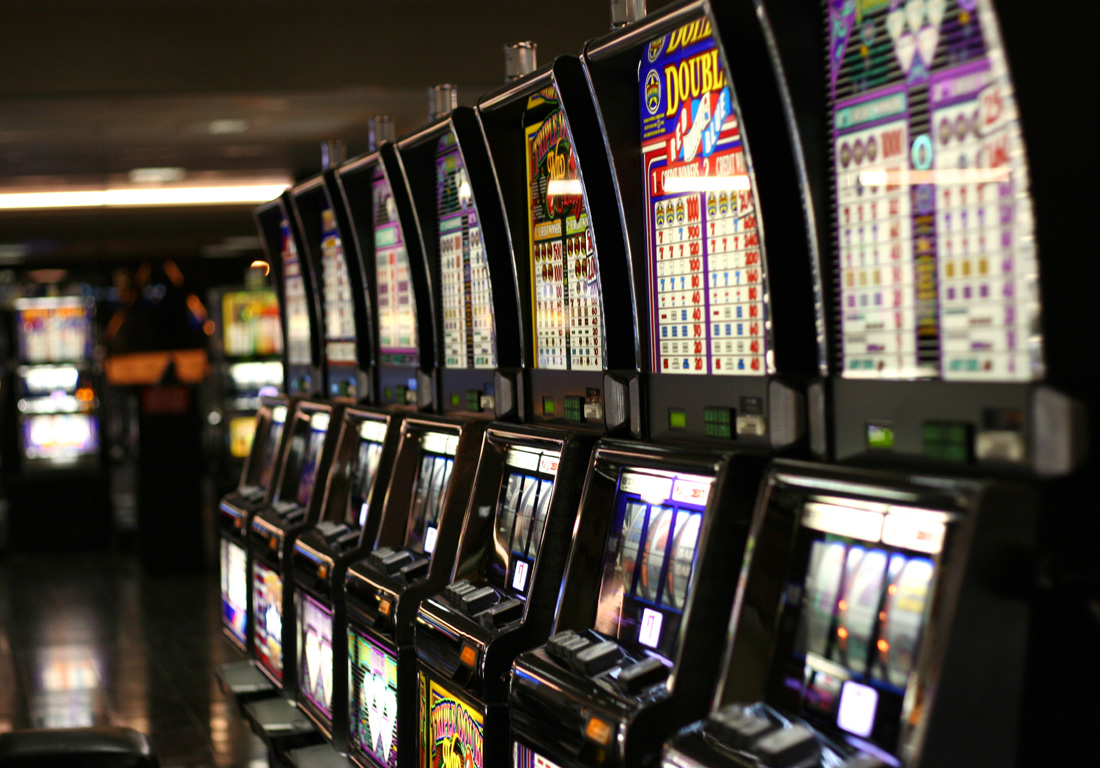
\includegraphics[width=3in]{images/Las_Vegas_slot_machines.eps}\\
    %% replicate charicature machine n times in a line
    So, what's the real question?
  }
\end{slide}

\begin{slide}{The Naive Approach}
  \begin{enumerate}
    \item Fix a trial budget
    \item Sample evenly from the machines
    \item Later pick the machine with the best payout with the rest of your cash
\end{enumerate}
\end{slide}

\begin{slide}{The Informal Model}
  Given a budget, determine which arm is best to pull and pull it as often as
  possible.\\ \pause
  \vspace{0.2in} Pull levers that aren't the best payout as infrequently as
  possible\\
  \vspace{0.2in}\pause
  But still be really sure that your notion of `best lever' is correct.
\end{slide}

\begin{slide}{The Formal Model}
  We have a set of bandits, modled by a set of distributions $B = {R_1, ..., R_K}$.\\\pause
  \vspace{0.2in}Each distribution $R_i$ represents the $i$th bandit, and has mean payout $\mu_i$.\\\pause
  \vspace{0.2in}We have a horizon $H$ which represents the number of pulls available to us.\\\pause
  \vspace{0.2in}The regret after $T$ rounds is $\rho = T\mu^* - \sum_{t=1}^{T}r_t$ where:\\
  $\mu^*$ is the mean payout of the best bandit, and $r_t$ is the reward earned
  from pull $t$.
\end{slide}

%%%%%%%%%%%%%%%%%%%%%%%%%%%%%%%%%%%%%%%%%%%%%%%%%%%%%%%%%%%%%%%%%%%%%
\section{Applied to Games}

\begin{slide}{But I Don't Want To Play Slots}
\end{slide}


\end{document}
